\chapter{من المواد الأولية إلى إعادة التدوير}\label{ch:g5:raw-materials-and-recycling}

تُرمى علبة مشروب فارغة في حاوية \omterm{def:g5:raw-materials-and-recycling:recycling}{إعادة التدوير}. فتنقلها شاحنة إلى مركز
للفرز، وتضغطها آلة في كتلة مع آلاف العلب الأخرى، ويصهر فرن الكتل، وبعد
بضعة أسابيع يعود المعدن إلى رفوف المتجر علبةً جديدة. فمن أين جاء المعدن
أصلًا، ولماذا يستحق الأمر أن نصهر العلب القديمة بدلًا من صنع معدن
جديد؟

\begin{recall}
الجسم شيء نراه ونلمسه؛ ومادته هي ما صُنع منه --- الخشب، والمعدن،
والزجاج، والبلاستيك، والورق، والقماش، والحجر
(\cref{ch:g1:materials-around-us}). وفي \omterm{def:g5:irreversible-changes:chemical-change}{التغير الكيميائي} تظهر مواد جديدة
ولا توجد طريق بسيطة للعودة (\cref{ch:g5:irreversible-changes}).
\end{recall}

\section{مواد طبيعية ومواد مصنّعة}

\begin{definition}[المواد الطبيعية والمواد المصنّعة]\label{def:g5:raw-materials-and-recycling:natural-material}
\emph{المادة الطبيعية}\index{مادة طبيعية} تُستعمل كما توجد في الطبيعة
تقريبًا، بعد قطعها أو تشكيلها فقط: الخشب، والحجر، والقطن، والصوف،
والجلد. أما \emph{المادة المصنّعة}\index{مادة مصنعة} فيصنعها الناس من
مواد موجودة في الطبيعة بعد تغييرها، وكثيرًا ما يكون ذلك بالحرارة
وبتغيرات كيميائية: الزجاج، والفولاذ، والألومنيوم، والبلاستيك، والورق،
والخرسانة.
\end{definition}

\begin{example}[طاولتان]\label{ex:g5:raw-materials-and-recycling:tables}
الطاولة المصنوعة من ألواح البلوط مصنوعة من \omterm{def:g5:raw-materials-and-recycling:natural-material}{مادة طبيعية}: فالخشب نُشر
وسُوّي وأُلصق فقط. أما الطاولة ذات السطح الزجاجي والأرجل الفولاذية
فمصنوعة من مواد مصنّعة: فلا الزجاج ولا الفولاذ يوجد على حاله في
الطبيعة.
\end{example}

\section{المواد الأولية}

\begin{definition}[المادة الأولية والخام]\label{def:g5:raw-materials-and-recycling:raw-material}
\emph{المادة الأولية}\index{مادة أولية} مادة تؤخذ من الطبيعة لصنع
المواد والأجسام: الأشجار، والرمل، والصخور، والنفط الخام، والقطن، والصوف.
والصخرة التي يُستخلص منها فلز تسمى
\emph{خامًا}\index{خام}.
\end{definition}

\begin{example}[من أين تأتي المواد]\label{ex:g5:raw-materials-and-recycling:from}
\begin{itemize}
  \item الخشب والورق يأتيان من الأشجار؛
  \item الزجاج يأتي من الرمل، بعد تسخينه تسخينًا شديدًا جدًا مع الصودا
        والحجر الجيري؛
  \item الحديد والفولاذ يأتيان من \omterm{def:g5:raw-materials-and-recycling:raw-material}{خام} الحديد، وهو صخرة ضاربة إلى الحمرة؛
  \item الألومنيوم يأتي من البوكسيت، وهو \omterm{def:g5:raw-materials-and-recycling:raw-material}{خام} آخر؛
  \item معظم أنواع البلاستيك يأتي من النفط الخام الذي يُضخ من باطن الأرض؛
  \item القطن يأتي من نبات، والصوف من الأغنام.
\end{itemize}
\end{example}

\begin{omfigure}
\begin{minipage}[b]{0.48\linewidth}\centering
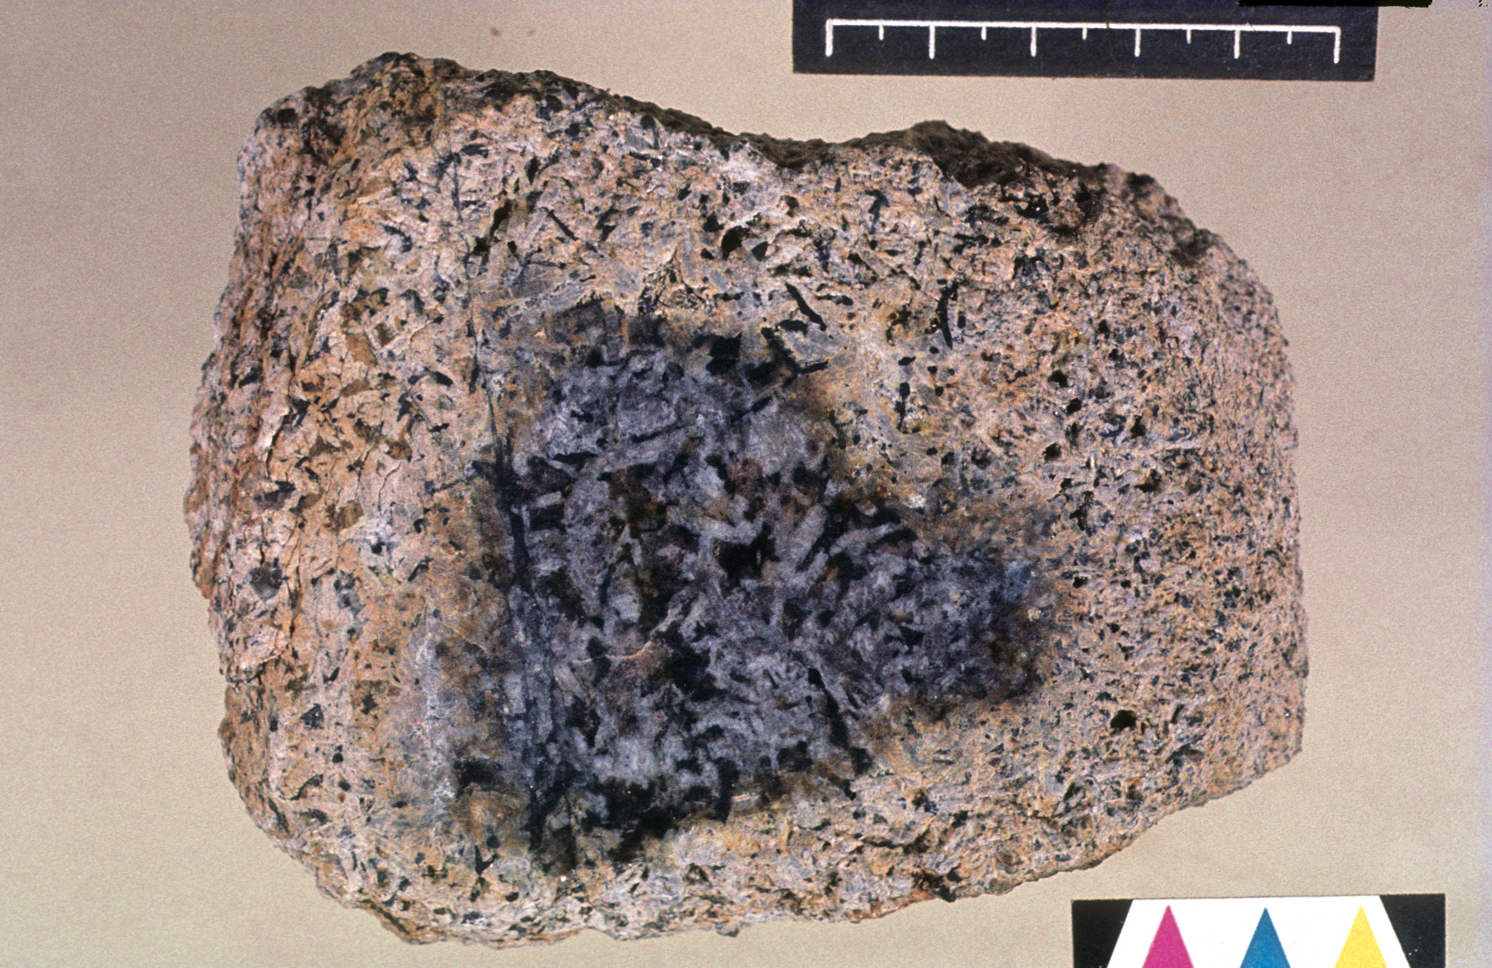
\includegraphics[width=\linewidth,height=4.6cm,keepaspectratio]{images/book1/bauxite.jpg}

{\small البوكسيت، \omterm{def:g5:raw-materials-and-recycling:raw-material}{خام} الألومنيوم، حول لبّ من صخر لم تتآكله
العوامل الجوية. تصوير: فيرنر شيلمان، CC BY-SA 2.5.}
\end{minipage}\hfill
\begin{minipage}[b]{0.48\linewidth}\centering
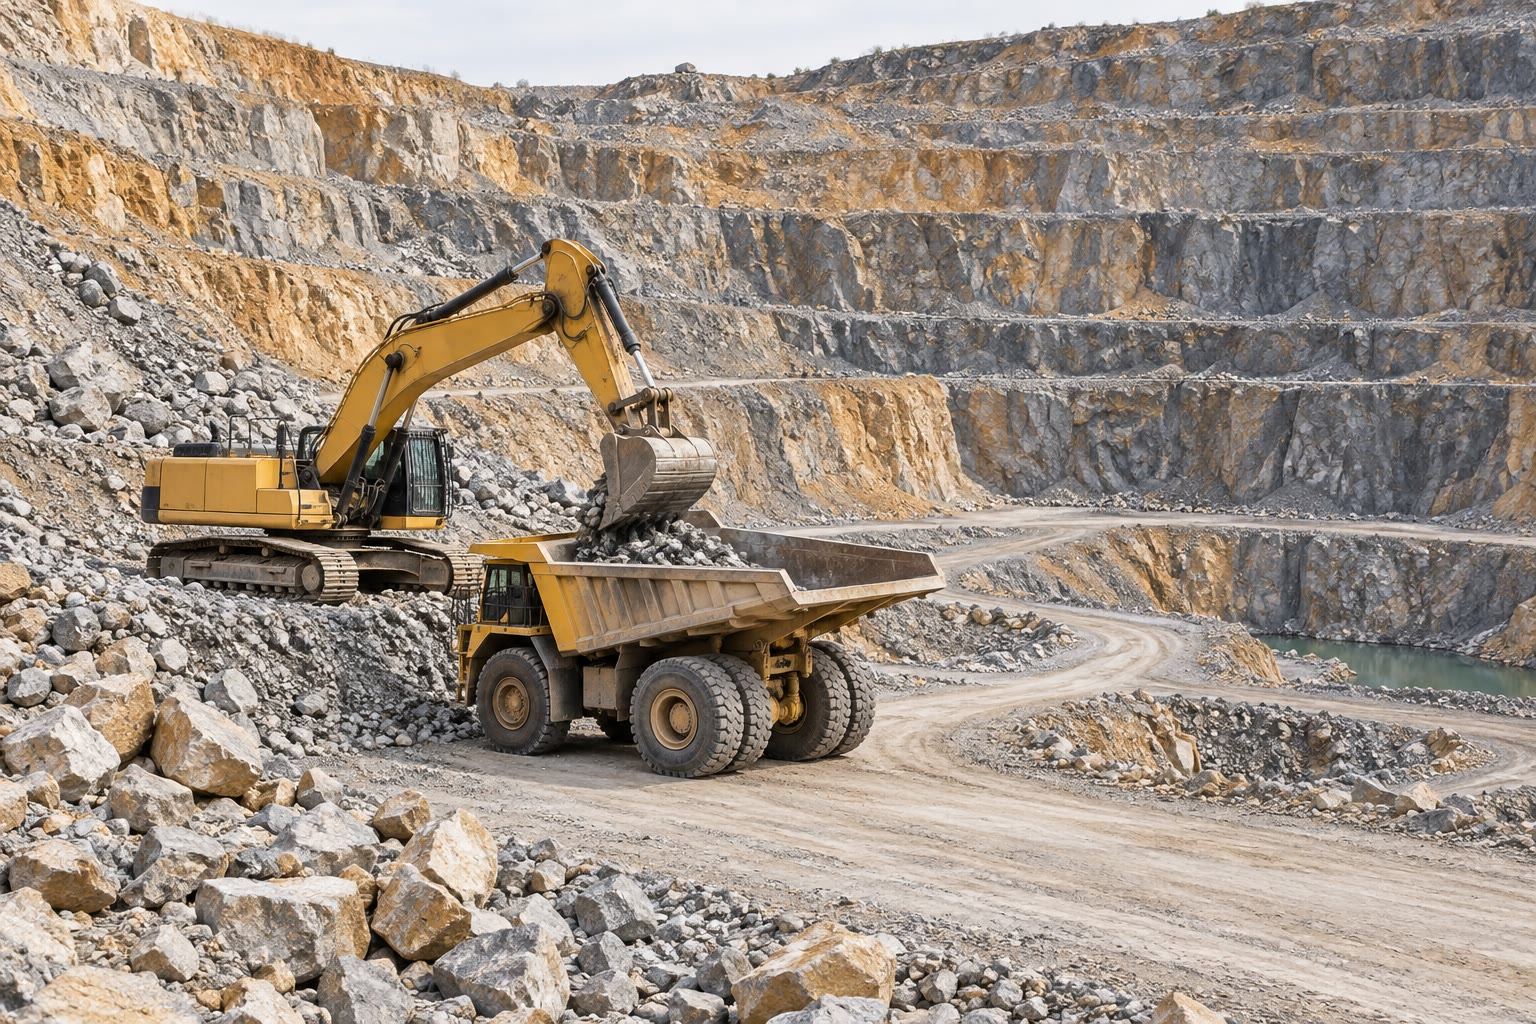
\includegraphics[width=\linewidth,height=4.6cm,keepaspectratio]{images/book1/ai/g5-quarry.jpg}

{\small مقلع: يُستخرج الصخر ليُستعمل مادةً أولية.}
\end{minipage}
\end{omfigure}

\begin{omfigure}
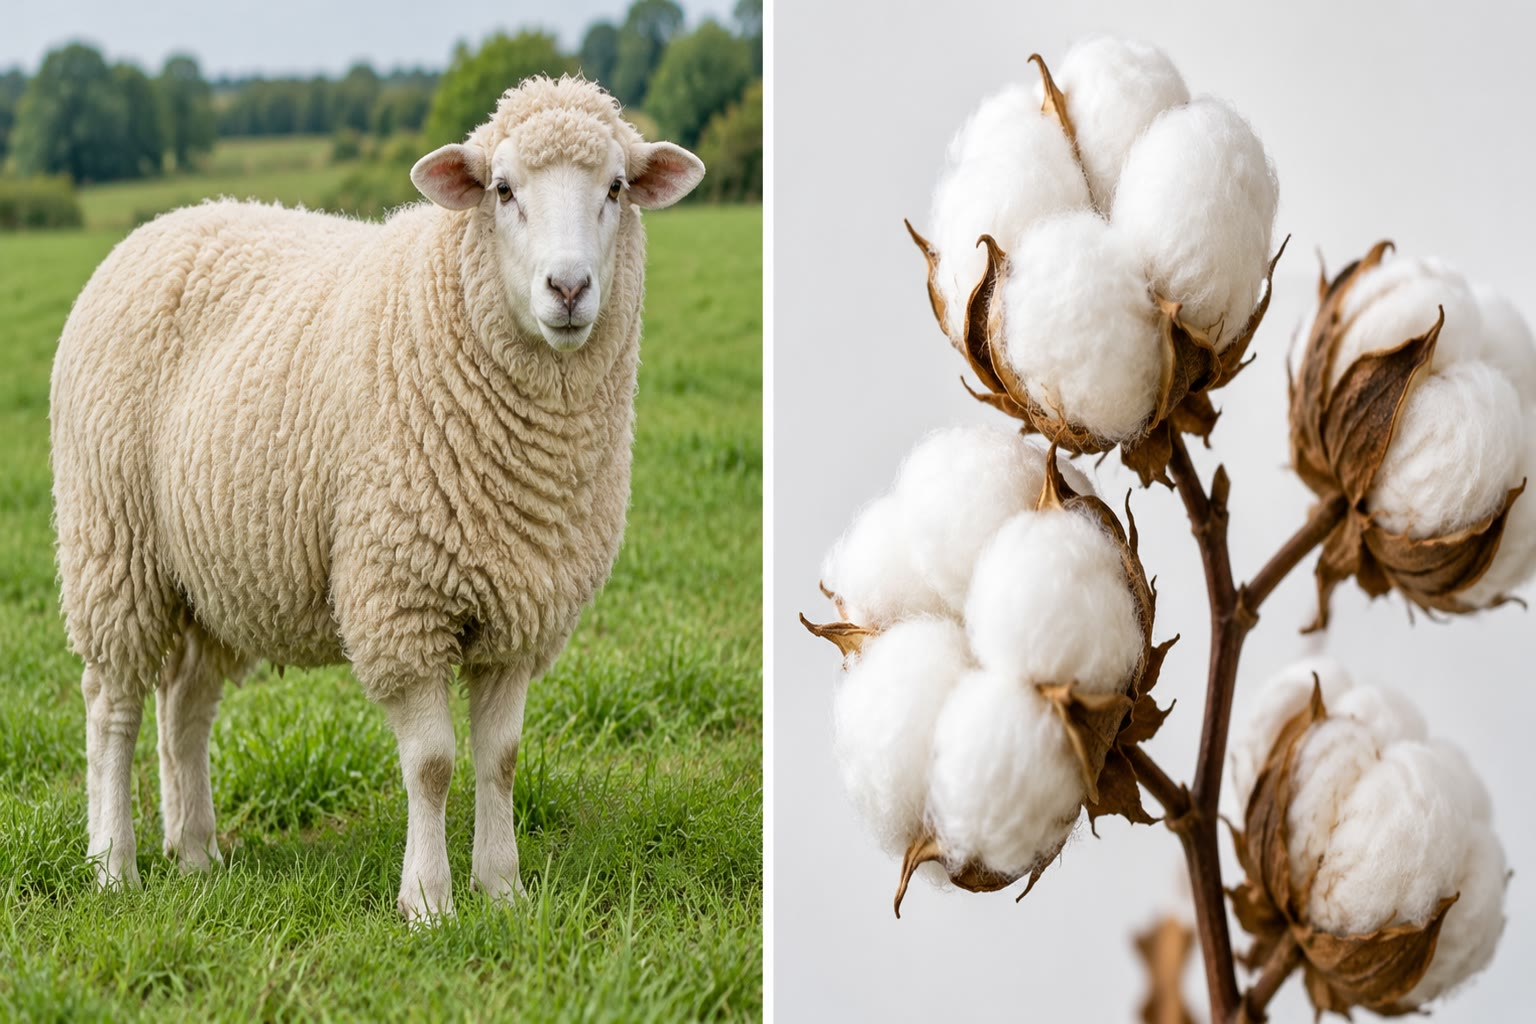
\includegraphics[width=0.6\linewidth]{images/book1/ai/g5-sheep-cotton.jpg}

{\small مواد أولية طبيعية من الكائنات الحية: الصوف من الأغنام،
والقطن من نبات القطن.}
\end{omfigure}

\section{من المادة الأولية إلى الجسم}

\begin{proposition}[صنع المادة يغيّر مادتها الأولية]\label{prop:g5:raw-materials-and-recycling:change}
يحتاج تحويل \omterm{def:g5:raw-materials-and-recycling:raw-material}{المادة الأولية} إلى مادة مصنّعة إلى طاقة --- هي في الغالب
حرارة فرن --- وإلى تغيرات كيميائية في العادة: فالرمل يصير زجاجًا، \omterm{def:g5:raw-materials-and-recycling:raw-material}{والخام}
يصير فلزًا، والنفط يصير بلاستيكًا. ولا يمكن الرجوع عن هذه التغيرات
ببساطة: فالزجاج لا يعود رملًا.
\end{proposition}

\begin{example}[حياة قارورة زجاجية]\label{ex:g5:raw-materials-and-recycling:bottle}
يُسخَّن الرمل والصودا والحجر الجيري المسحوق معًا في فرن حتى تنصهر فتصير
زجاجًا. ثم يُنفخ الزجاج الساخن على شكل قارورة. تُملأ القارورة وتُباع
وتُفرغ. فإذا وُضعت في حاوية الزجاج كُسرت قطعًا صغيرة، وصُهرت من جديد،
ونُفخت قارورةً جديدة: فيُستعمل الزجاج مرة بعد مرة.
\end{example}

\begin{omfigure}
\begin{tikzpicture}[font=\small,
    box/.style={draw=omDef, fill=omDef!6, rounded corners=2pt, align=center,
      minimum height=0.95cm, text width=2.4cm}]
  \node[box] (r) at (0,2.6) {مادة أولية\\ (رمل، خام، نفط)};
  \node[box] (m) at (4.0,2.6) {صنع\\ المادة};
  \node[box] (o) at (8.0,2.6) {جسم\\ مستعمل};
  \node[box] (w) at (8.0,0) {نفايات};
  \node[box, draw=omProp, fill=omProp!8] (s) at (4.0,0) {الفرز وإعادة\\ التدوير};
  \draw[->, thick, omDef] (r) -- (m);
  \draw[->, thick, omDef] (m) -- (o);
  \draw[->, thick, omDef] (o) -- (w);
  \draw[->, thick, omProp] (w) -- (s);
  \draw[->, thick, omProp] (s) -- (m) node[midway, left, align=right, text=black]
    {تُستعمل من جديد\\ بدلًا من مادة\\ أولية جديدة};
  \draw[->, thick, black!45, dashed] (w.east) -- ++(1.4,0) node[right, align=left,
    text=black] {تُرمى:\\ في المكبّ};
\end{tikzpicture}

{\small حياة مادة. الحلقة البرتقالية هي \omterm{def:g5:raw-materials-and-recycling:recycling}{إعادة التدوير}: مادة جسم قديم
تحل محل \omterm{def:g5:raw-materials-and-recycling:raw-material}{مادة أولية} جديدة.}
\end{omfigure}

\section{الفرز وإعادة التدوير}

\begin{definition}[إعادة التدوير]\label{def:g5:raw-materials-and-recycling:recycling}
\emph{إعادة التدوير}\index{إعادة التدوير} جمع الأجسام المستعملة ومعالجة
مادتها كي تُصنع منها أجسام جديدة، بدلًا من رميها.
\end{definition}

\begin{proposition}[لماذا نعيد التدوير]\label{prop:g5:raw-materials-and-recycling:why}
% ledger: al:energy-primary, al:energy-recycled (8.3 / 186 = about 1/22)
\omterm{def:g5:raw-materials-and-recycling:recycling}{إعادة التدوير} توفر المواد الأولية، فلا حاجة إلى استخراجها من باطن الأرض،
وكثيرًا ما توفر الطاقة. فصنع الألومنيوم من العلب القديمة لا يتطلب إلا
نحو جزء من عشرين من الطاقة اللازمة لصنعه من البوكسيت. وهي تعني أيضًا
نفايات أقل في المكبّات.
\end{proposition}

\begin{method}[فرز النفايات لإعادة التدوير]\label{met:g5:raw-materials-and-recycling:sort}
تبدأ \omterm{def:g5:raw-materials-and-recycling:recycling}{إعادة التدوير} بالفرز، حيثما تُرمى النفايات:
\begin{enumerate}
  \item القوارير والمرطبانات الزجاجية في حاوية واحدة؛
  \item العلب المعدنية، والورق والورق المقوى، والقوارير البلاستيكية في
        الحاويات التي توفرها المدينة لها (وتختلف ألوان الحاويات من
        مكان إلى آخر)؛
  \item وما لا يمكن تدويره مع بقية النفايات.
\end{enumerate}
يُعاد تدوير كل مادة بطريقتها الخاصة، ولذلك يجب ألا تحوي الحاوية إلا
المواد المخصصة لها.
\end{method}

\begin{omfigure}
\begin{tikzpicture}[font=\small]
  \foreach \k/\t/\bc in {0/{زجاج}/green!50!black, 1/{علب معدنية}/gray,
                        2/{ورق وورق مقوى}/omDef, 3/{قوارير بلاستيكية}/orange!80!black} {
    \begin{scope}[xshift=\k*3.4cm]
      \fill[\bc!18, draw=\bc, line width=0.8pt] (-1,0) -- (1,0) -- (1.15,2.0)
        -- (-1.15,2.0) -- cycle;
      \fill[\bc!45, draw=\bc] (-1.25,2.0) rectangle (1.25,2.3);
      \node[anchor=north, align=center] at (0,-0.15) {\t};
    \end{scope}
  }
  % glass: a bottle
  \fill[green!40!black!60] (-0.2,0.3) rectangle (0.2,1.2);
  \fill[green!40!black!60] (-0.07,1.2) rectangle (0.07,1.6);
  % metal: a can
  \begin{scope}[xshift=3.4cm]
    \fill[black!25, draw=black!55] (-0.3,0.3) rectangle (0.3,1.3);
  \end{scope}
  % paper: a box and a sheet
  \begin{scope}[xshift=6.8cm]
    \fill[brown!25, draw=brown!60] (-0.6,0.3) rectangle (0.1,1.0);
    \fill[white, draw=black!40] (0.2,0.3) rectangle (0.65,1.3);
  \end{scope}
  % plastic: a bottle
  \begin{scope}[xshift=10.2cm]
    \fill[cyan!20, draw=cyan!50!black] (-0.25,0.3) rectangle (0.25,1.3);
    \fill[cyan!20, draw=cyan!50!black] (-0.1,1.3) rectangle (0.1,1.6);
  \end{scope}
\end{tikzpicture}

{\small أربع حاويات للفرز، واحدة لكل مادة. (تختلف ألوان الحاويات
الحقيقية من مدينة إلى أخرى.)}
\end{omfigure}

\begin{omfigure}
\begin{minipage}[t]{0.48\linewidth}\centering
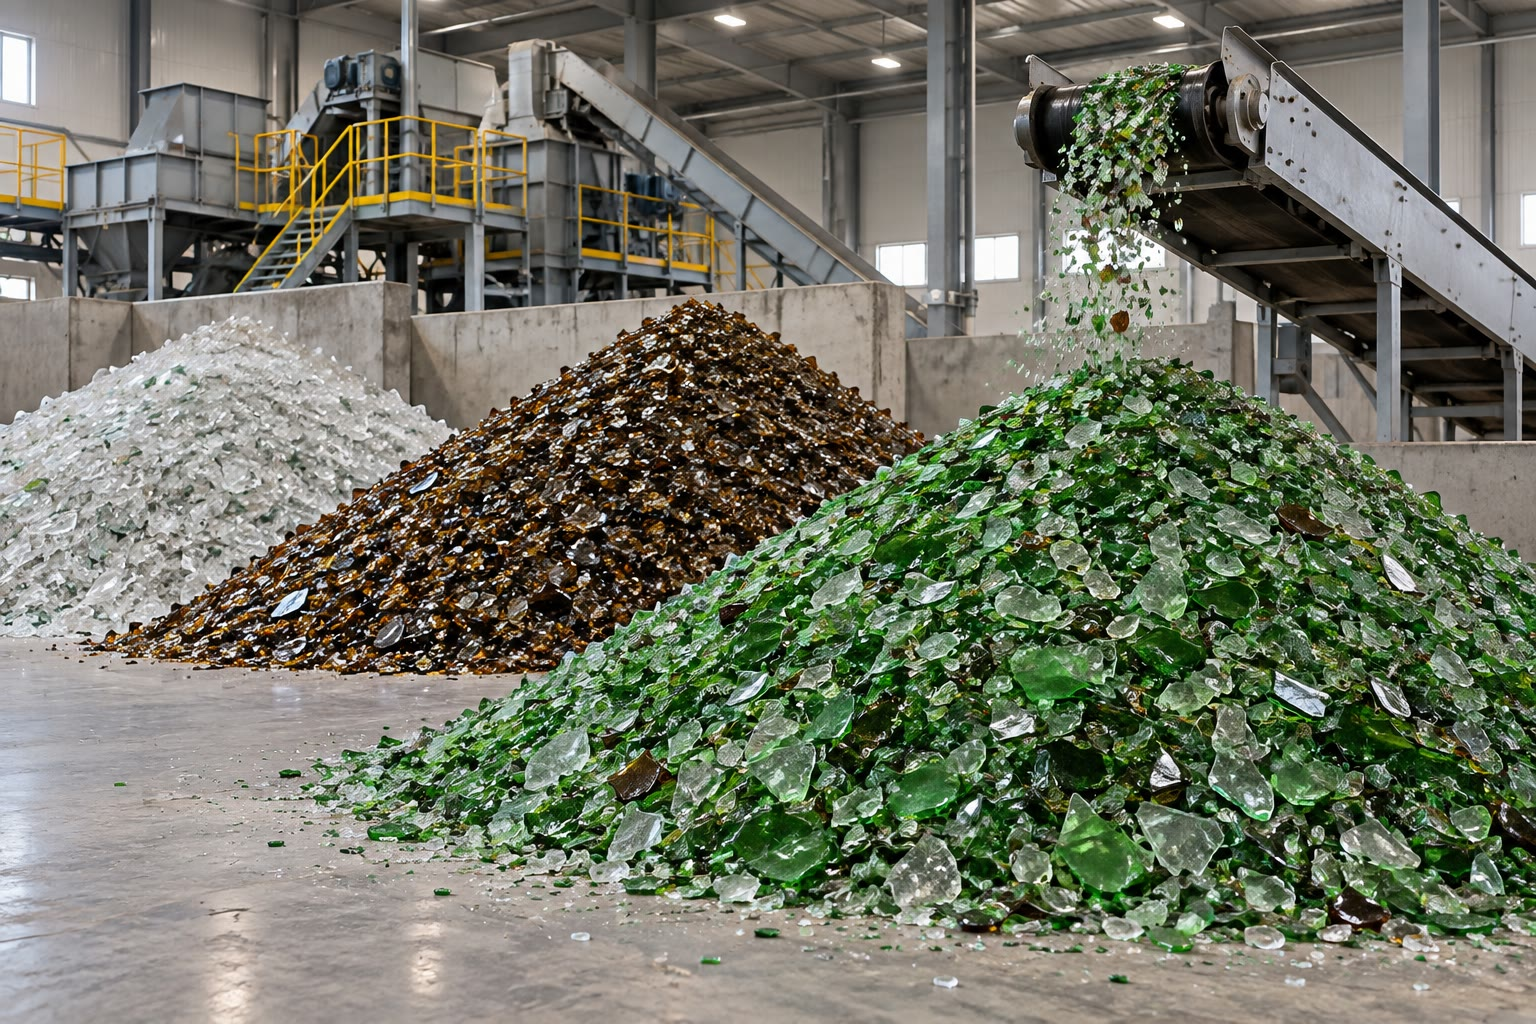
\includegraphics[width=\linewidth,height=4.6cm,keepaspectratio]{images/book1/ai/g5-glass-cullet.jpg}

{\small زجاج مكسّر في مصنع \omterm{def:g5:raw-materials-and-recycling:recycling}{لإعادة التدوير}، جاهز للصهر.}
\end{minipage}\hfill
\begin{minipage}[t]{0.48\linewidth}\centering
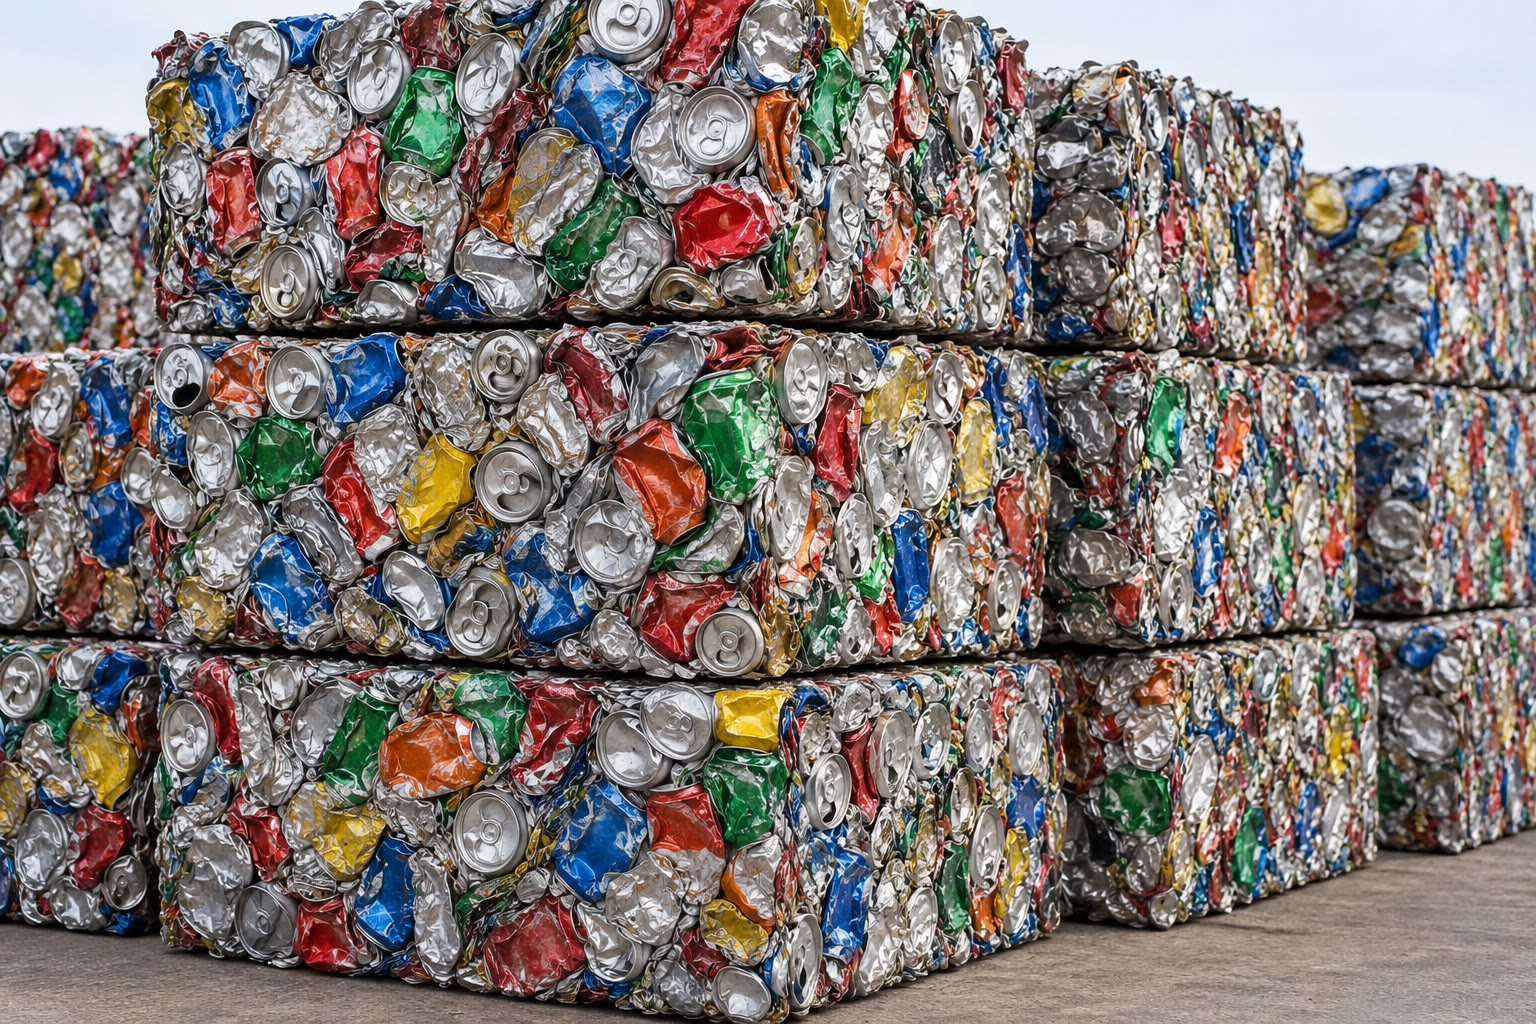
\includegraphics[width=\linewidth,height=4.6cm,keepaspectratio]{images/book1/ai/g5-can-bales.jpg}

{\small رزم من علب الألومنيوم المضغوطة.}
\end{minipage}
\end{omfigure}

\section{النفايات والموارد}

\begin{definition}[المورد]\label{def:g5:raw-materials-and-recycling:resource}
\emph{المورد}\index{مورد} كل ما يؤخذ من الطبيعة ويستعمله الناس: الماء،
والخشب، والخامات، والنفط، والرمل. و\emph{المورد
المتجدد}\index{مورد متجدد} ينمو من جديد أو يعود من تلقاء نفسه في
حدود عمر الإنسان، مثل خشب غابة يُعاد تشجيرها أو صوف الأغنام. أما الخامات
والنفط الخام فليست متجددة: فإذا استُخرجت واستُعملت ذهبت.
\end{definition}

\begin{proposition}[قلّل، وأعد الاستعمال، وأعد التدوير]\label{prop:g5:raw-materials-and-recycling:three}
لكي تدوم الموارد، يستطيع الناس، بهذا الترتيب:
\begin{enumerate}
  \item \textbf{التقليل}: استعمال أجسام أقل، مثل تقليل
        الأغلفة؛
  \item \textbf{إعادة الاستعمال}: استعمال الجسم نفسه مرة أخرى، مثل
        مرطبان زجاجي يُعاد ملؤه أو كيس يُحمل من جديد إلى المتجر؛
  \item \textbf{\omterm{def:g5:raw-materials-and-recycling:recycling}{إعادة التدوير}}: تحويل المادة إلى جسم جديد.
\end{enumerate}
وتأتي \omterm{def:g5:raw-materials-and-recycling:recycling}{إعادة التدوير} في الأخير لأنها لا تزال تحتاج إلى طاقة وآلات؛ وخير
النفايات ما لا يُصنع أبدًا.
\end{proposition}

\section{تمارين}

\begin{exercise}[$\star$]\label{exo:g5:raw-materials-and-recycling:1}
طبيعية أم مصنّعة؟ الخشب، والزجاج، والصوف، والفولاذ، والبلاستيك، والحجر.
\end{exercise}

\begin{exercise}[$\star$]\label{exo:g5:raw-materials-and-recycling:2}
اذكر \omterm{def:g5:raw-materials-and-recycling:raw-material}{المادة الأولية} لكل من: ورقة، ومرطبان زجاجي، وقميص قطني، وقارورة
بلاستيكية.
\end{exercise}

\begin{exercise}[$\star$]\label{exo:g5:raw-materials-and-recycling:3}
ما \omterm{def:g5:raw-materials-and-recycling:raw-material}{الخام}؟ سمِّ \omterm{def:g5:raw-materials-and-recycling:raw-material}{خام} الألومنيوم.
\end{exercise}

\begin{exercise}[$\star$]\label{exo:g5:raw-materials-and-recycling:4}
في أي حاوية تضع: مرطبان مربى فارغًا، وجريدة، وعلبة مشروب، وقارورة ماء
بلاستيكية؟
\end{exercise}

\begin{exercise}[$\star$]\label{exo:g5:raw-materials-and-recycling:5}
انظر إلى شكل حياة المادة. ماذا تحل الحلقة البرتقالية
محله؟
\end{exercise}

\begin{exercise}[$\star$]\label{exo:g5:raw-materials-and-recycling:6}
متجدد أم لا: الخشب، والنفط الخام، والصوف، \omterm{def:g5:raw-materials-and-recycling:raw-material}{وخام} الحديد، والقطن؟
\end{exercise}

\begin{exercise}[$\star$]\label{exo:g5:raw-materials-and-recycling:7}
لماذا لا يمكن أن يعود الزجاج رملًا بتبريده؟
\end{exercise}

\begin{exercise}[$\star$]\label{exo:g5:raw-materials-and-recycling:8}
أعطِ طريقة للتقليل، وطريقة لإعادة الاستعمال، وطريقة \omterm{def:g5:raw-materials-and-recycling:recycling}{لإعادة التدوير}.
\end{exercise}

\begin{exercise}[$\star$]\label{exo:g5:raw-materials-and-recycling:9}
لماذا يجب ألا تحوي حاوية الزجاج إلا الزجاج؟
\end{exercise}

\begin{exercise}[$\star\star$]\label{exo:g5:raw-materials-and-recycling:10}
صنع الألومنيوم من العلب القديمة يتطلب نحو جزء من عشرين من الطاقة اللازمة
لصنعه من البوكسيت. يستهلك مصنع 20 وحدة من الطاقة لصنع دفعة من
الألومنيوم من البوكسيت. كم وحدة تقريبًا يستهلك لصنع الدفعة نفسها من
العلب القديمة؟
\end{exercise}

\begin{exercise}[$\star\star$]\label{exo:g5:raw-materials-and-recycling:11}
لماذا يأتي «التقليل» قبل «\omterm{def:g5:raw-materials-and-recycling:recycling}{إعادة التدوير}»؟
\end{exercise}
